
\documentclass[letterpaper, reqno,11pt]{article}
\usepackage[margin=1.0in]{geometry}
\usepackage{color,latexsym,amsmath,amssymb}
\usepackage{fancyhdr}
\usepackage{amsthm}
\usepackage{mathtools}
\usepackage{tikz}
\usepackage{float}
\usepackage{centernot}
\usepackage{subcaption}
\usepackage{extarrows}
\usetikzlibrary{hobby}
\usetikzlibrary{shapes.multipart}
\usepackage{pgfplots}
\pgfplotsset{compat=1.7}
\usetikzlibrary{arrows.meta}

\newcommand{\RR}{\mathbb{R}}
\newcommand{\CC}{\mathbb{C}}
\newcommand{\ZZ}{\mathbb{Z}}
\newcommand{\QQ}{\mathbb{Q}}
\newcommand{\NN}{\mathbb{N}}
\def\upint{\mathchoice%
  {\mkern13mu\overline{\vphantom{\intop}\mkern7mu}\mkern-20mu}%
  {\mkern7mu\overline{\vphantom{\intop}\mkern7mu}\mkern-14mu}%
  {\mkern7mu\overline{\vphantom{\intop}\mkern7mu}\mkern-14mu}%
  {\mkern7mu\overline{\vphantom{\intop}\mkern7mu}\mkern-14mu}%
  \int}
\def\lowint{\mkern3mu\underline{\vphantom{\intop}\mkern7mu}\mkern-10mu\int}
\DeclareMathOperator{\card}{card}
\DeclareMathOperator{\Binomial}{Binomial}
\pagestyle{fancy}
\lhead{Math 321 Lecture 16}
\rhead{Yuchong Pan}
\begin{document}
\pagenumbering{arabic}
\title{Math 321 Lecture 16}
\author{Yuchong Pan}
\date{February 8, 2019}
\newtheorem{thm}{Theorem}
\newtheorem{defn}{Definition}
\newtheorem*{remark}{Remark}
\newtheorem{claim}{Claim}
\newtheorem{cor}{Corollary}
\newtheorem{lemma}{Lemma}
\newtheorem{prop}{Proposition}
\maketitle
%

\section{Theorem}

\begin{thm}
  \normalfont $\mathcal R_\alpha[a, b]$ is closed under uniform convergence; i.e., if $\{ f_n : n \geq 1 \} \subseteq \mathcal R_\alpha[a, b]$ and $f_n \xrightarrow{n \to \infty} f$ uniformly on $[a, b]$, then $f \in \mathcal R_\alpha[a, b]$ and $\int_a^b f_n d\alpha \xrightarrow{n \to \infty} \int_a^b fd\alpha$.
\end{thm}

\begin{proof}
  \noindent {\bf Step 1:} To show that $f \in \mathcal R_\alpha[a, b]$. Will invoke Riemann's condition for this. Fix $\epsilon > 0$. Need to find a partition $P = P_\epsilon$ such that $U_\alpha(f, P) - L_\alpha(f, P) < \epsilon$.

  For any partition $Q$ of $[a, b]$,
  $$ U_\alpha(f, Q) - L_\alpha(f, Q) = \sum_{i = 1}^n \underbrace{\omega(f, I_i)}_{= (M_i - m_i)} \omega(\alpha, I_i), $$
  where
  $$ Q = \{ x_0 = a < x_1 < \ldots < x_n = b \}, \qquad I_i = [x_{i - 1}, x_i]. $$

  \noindent {\bf Recall:}
  \begin{align}
    & \text{$f_n \xrightarrow{n \to \infty} f$ uniformly if and only if} \nonumber \\
    \Leftrightarrow ~ & \exists N \text{ s.t. } \sup_{x \in [a, b]} |f_n(x) - f(x)| < \frac{\epsilon}{10} ~ \forall n \geq N. \label{eq:1}
  \end{align}
  Choose $n = N$.
  \begin{align*}
    |f(s) - f(t)| &\overset{\text{triangular inequality}}{\leq} \underbrace{|f_n(s) - f(s)|}_{< \frac{\epsilon}{10} \text{ by \eqref{eq:1}}} + \underbrace{|f_n(t) - f(t)|}_{< \frac{\epsilon}{10} \text{ by \eqref{eq:1}}} + |f_n(s) - f_n(t)| \\
    &< \frac{\epsilon}{5} + |f_n(s) - f_n(t)|.
  \end{align*}

  If $s, t \in I_i = [x_{i - 1}, x_i]$, then the above implies
  \begin{equation} \label{eq:*} \tag{*}
    \omega(f, I_i) \leq \omega(f_n, I_i) + \frac{\epsilon}{5}.
  \end{equation}
  Use \eqref{eq:*}.
  \begin{equation} \label{eq:**} \tag{**}
    U_\alpha(f, Q) - L_\alpha(f, Q) \leq \sum_{i = 1}^n \left(\frac{\epsilon}{5} + \omega(f_N, I_i)\right) \omega(\alpha, I_i).
  \end{equation}
  Note that
  $$ \omega(f, I_i) = \sup\{ |f(s) - f(t)| : s, t \in I_i \}, $$
  where
  $$ |f(s) - f(t)| < \frac{\epsilon}{5} + |f_n(s) - f_n(t)| \leq \underbrace{\frac{\epsilon}{5} + \overbrace{\omega(f_n, I_i)}^\text{independent of $s, t$}}_\text{an upper bound for $\{ |f(s) - f(t)| : s, t \in I_i \}$}. $$
  This implies that
  $$ \underbrace{\omega(f, I_i)}_\text{least upper bound} \leq \frac{\epsilon}{5} + \omega(f_n, I_i). $$
  Choose the partition $Q = P_N$ such that
  $$ U_\alpha(f_N, P_N) - L_\alpha(f_N, P_N) < \frac{\epsilon}{5}. $$
  Such a partition $P_N$ exists by Riemann's condition, since $f_N \in \mathcal R_\alpha[a, b]$.
  \begin{align*}
    U_\alpha(f, P_N) - L_\alpha(f, P_N) &\leq \frac{\epsilon}{5} \sum_{i = 1}^n \omega(\alpha, I_i) + \underbrace{[U_\alpha(f_N, P_N) - L_\alpha(f_N, P_N)]}_{< \frac{\epsilon}{5}} \\
    &= \frac{\epsilon}{5} \underbrace{(\alpha(b) - \alpha(a))}_{C_\epsilon} + \frac{\epsilon}{5}.
  \end{align*}

  \noindent {\bf Step 2:} To show that
  \begin{align*}
    & \int_a^b f_n d\alpha \xrightarrow{n \to \infty} \int_a^b fd\alpha \\
    \Leftrightarrow ~ & \int_a^b (f_n - f) d\alpha \xrightarrow{n \to \infty} 0.
  \end{align*}
  Use $\lVert f_n - f \rVert_\infty < \epsilon$ for all $n \geq N$ to show
  $$ \left|\int_a^b (f_n - f) d\alpha\right| \underbrace{\leq}_\text{Justify!} \int_a^b |f_n - f| d\alpha < \epsilon \int_a^b d\alpha = \epsilon (\alpha(b) - \alpha(a)). $$
\end{proof}

\section{Bounded Variation}

\begin{remark}
  \normalfont So far:
  \begin{enumerate}
  \item We have defined $\int_a^b fd\alpha$ only on compact intervals $[a, b]$.
  \item Depends on $\alpha$.
  \item Computability issues?
  \item Immediate applications to physical problems are unclear.
  \item Can $\int_a^x fd\alpha$ be interpreted as some kind of antiderivative?
  \end{enumerate}
\end{remark}

\noindent {\bf Example:} Let $\Gamma = \left\{ e^{i\theta} : \theta \in [0, 2\pi] \right\}$.

\begin{figure}[H]
  \centering
  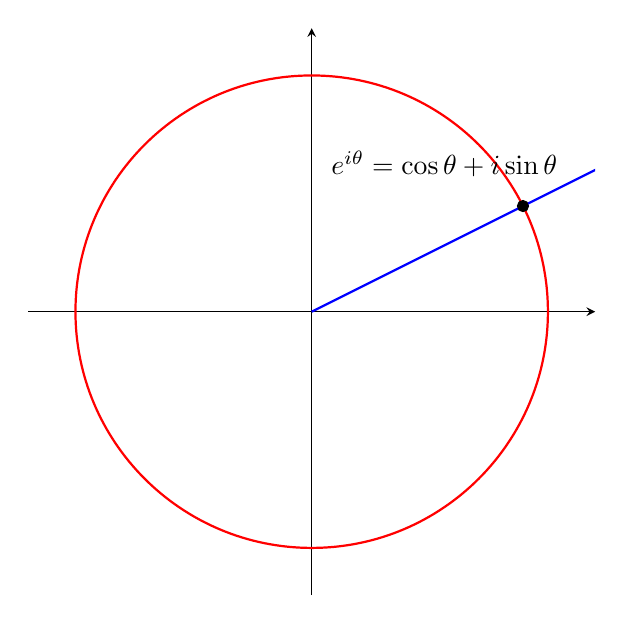
\begin{tikzpicture}
    \begin{axis}[
        xmin=-1.2,
        xmax=1.2,
        ymin=-1.2,
        ymax=1.2,
        xmajorticks=false,
        ymajorticks=false,
        axis x line=center,
        axis y line=center,
        x=3cm,
        y=3cm,
      ]
      \draw[red, thick] (axis cs: 0, 0) circle (1);
      \addplot[thick, blue, samples at={0, 0.05, ..., 2}](x,{0.5*x});
      \draw[fill=black] (axis cs:0.8944, 0.4472) circle (2pt) node [above, xshift=-1cm, yshift=0.25cm] {$e^{i\theta} = \cos\theta + i\sin\theta$};
    \end{axis}
  \end{tikzpicture}
\end{figure}

\noindent {\bf Note:} A typical path integral
$$ \int_P f\underbrace{dz}_\text{integral of $f$ on $\Gamma$}. $$
does not correspond to any $\mathcal R_\alpha[a, b]$ developed so far.

\medskip

\noindent Need to expand our class of integrators.

\begin{defn}
  \normalfont Let $\alpha : [a, b] \to \RR$. Let $P$ be a partition of $[a, b]$. Define
  $$ V_a^b (\alpha, P) = \sum_{i = 1}^n |\alpha(x_i) - \alpha(x_{i - 1})|. $$
  The {\bf total variation} of $\alpha$ on $[a, b]$ is defined as
  $$ V_a^b (\alpha) = \sup_P V_a^b (\alpha, P). $$
  Call $\alpha = BV[a, b]$ if $V_a^b (\alpha) < \infty$.
\end{defn}

\noindent {\bf Show:} $V_a^b (\alpha, P) \leq V_a^b (\alpha, Q)$ if $P \subseteq Q$.

\end{document}
